\subsection{Resistor-Capacitor Circuits}\label{sec:resistor_capcitor_circuits}

\begin{figure}[H]
    \centering
    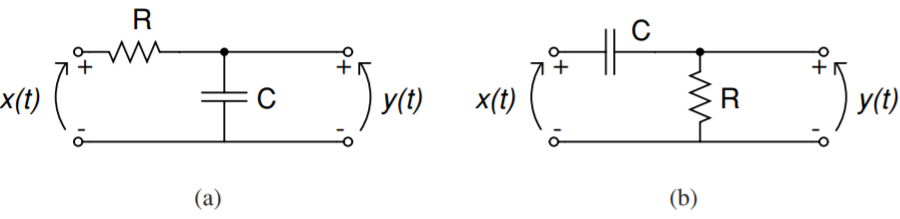
\includegraphics[width=0.8\linewidth]{../../Figures/RC_Circuits.PNG}
    \caption{Resistor capacitor (RC) circuits. The signals $x(t)$ represent input voltages, and the signals $y(t)$ represent output voltages. (a) Integrator circuit (low pass filter); (b) Differentiator circuit (high pass filter). Adapted from textbook}
    \label{fig:RC_Circuits}
\end{figure}

I advise finding a memory hack to remember which is which. I know I begin with RC (not CR) which is low (you begin low and then you go high) and treats the "primitive" (integrator).   

\subsubsection{Solving Low pass Integrator RC circuit}

Figure \ref{fig:RC_Circuits}.a). Let's start by analyzing the circuit in a), and we need to start with KCL voltage law: 
\begin{equation}
    u_{in} = u_R + u_C, 
\end{equation}

where $u_R$ and $u_C$ are the voltage drops over the resistor $R$ and capacitor $C$, respectively. 

We have some current flowing in the branch (assuming no current is flowing out of the main branch, so no current in y(t)). According to Ohm's law we have: NEED TO EXPLAIN THIS: 
\begin{equation}
    u_R = i.R \mathrm{, and }\ u_C = \frac{i}{j\omega C} 
\end{equation}
When combining these two equations, we get: 
\begin{equation}
    u_{in} = i\cdot R + i\cdot \frac{1}{j \omega C} = i \cdot (R + \frac{1}{j \omega C})
\end{equation}

In the case of this circuit, because voltage is the same across parallel branches, $u_{out} = u_c$, we can therefore write the transfer function $\frac{u_{out}}{u_{in}}$ as follows: 

\begin{equation}
    \frac{u_{out}}{u_{in}} = \frac{i \cdot 1/j \omega C}{i \cdot (R + 1/j \omega C)} = \frac{1}{j \omega RC + 1}
\end{equation}

Now we can rearrange and essentially obtain a differential equation (remembering that $\frac{de^{j\omega t}}{dt} = j \omega e^{j\omega t}$)

\begin{equation}
    j \omega \cdot RC u_{out} + u_{out} = u_{in} \equiv RC\frac{du_{out}}{dt} + u_{out} = u_{in}
\end{equation}

You may wonder what this is all about, and why am I even doing this. I wondered myself, but don't worry, we'll get to it. It's all about transfer functions and understanding how the system output changes with respect to input change.

One important thing, $RC$ has now appeared. As you can see, it is a constant (assuming resistance and capacitance are constant in a circuit) that scales the rate of change of the output with respect to time. This is called the time constant and is noted $\tau$ . This is critically important to understand charging and discharging time of capacitors (see Figure \ref{fig:Time_Constant}.The formal definition is: The circuit's time constant $\tau = RC$ is the time required to discharge the capacitor, through the resistor, to 36.8\% (1/e) of its final steady state value.

\begin{figure}[H]
    \centering
    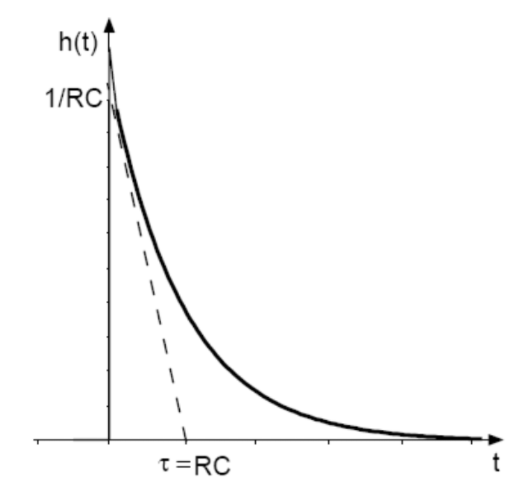
\includegraphics[width=0.4\linewidth]{../../Figures/RC_Time_Constant.PNG}
    \caption{The circuit's time constant $\tau = RC$ is the time required to discharge the capacitor, through the resistor, to 36.8\% (1/e) of its final steady state value. Adapted from lecture notes}
    \label{fig:Time_Constant}
\end{figure}



\begin{equation}
    H(s) = \frac{Y(s)}{X(s)} = \frac{1}{1 + RCj \omega }
\end{equation}

\paragraph{Solving with Laplace transform}

In Laplace domain, the equation can be rearranged to: 
\begin{equation}
    \tau s Y(s) + Y(s) = X(s)
\end{equation}

We can now also conveniently define the transfer function $H(s)$, taking $X(s) = 1$ (impulse): 

\begin{equation}
    H(s) = \frac{Y(s)}{X(s)} = \frac{1}{1 + \tau s}
\end{equation}


\subsubsection{Solving High pass Differentiator CR circuit} 

Figure \ref{fig:RC_Circuits}.b). I won't be going into the derivation for this, but it really follows the same logic. In the end, we reach this differential equation: 

\begin{equation}
    j \omega \cdot \tau \cdot u_{out} + u_{out} = u_{in} \equiv \tau \frac{du_{out}}{dt} + u_{out} = \tau\frac{d u_{in}}{dt}
\end{equation}

\paragraph{Solving with Laplace transform}

In Laplace domain, the equation can be rearranged to: 

\begin{equation}
    \tau s Y(s) + Y(s) = sX(s)
\end{equation}

Yielding the transfer function (also taking $X(s) = 1$): 

\begin{equation}
    H(s) = \frac{Y(s)}{X(s)} = \frac{\tau s}{1 + \tau s }
\end{equation}

\subsubsection{Frequency Domain Analysis}

It may not be clear yet to you why are these circuits called lowpass/high pass filters, as well as differentiator/integrators. While we will look at the differentiator/integrator property in the next circuit, we can first start with some frequency domain analysis to make the filtering part clearer. 

Let's now consider how this circuit responds to sinusoidal signals of different \textit{frequencies}. Sinusoids have a very special relationship to shift-invariant linear systems, such as the one we are analyzing. When a sinusoidal signal is applied as input to a shift-invariant linear system, then its response will be another sinusoidal signal, with possibly a different amplitude and a different phase, but certainly with exactly the same frequency! That is, if the input is $x(t) = \mathrm{sin}(\omega t)$, the output will be $y(t) = A \mathrm{sin}(\omega t + \phi)$, where A and $\phi$ determine the scaling and shift.

Remember that the transfer function we obtained earlier for the RC low pass filter circuit was $H(s) = \frac{Y(s)}{X(s)} = \frac{1}{1 + \tau s}$. This is in Laplace domain, if we are playing with frequencies of signals, it makes sense to switch to the frequency (time) domain. In this domain $s = j \omega$ and the circuit's transfer function simply becomes: 

\begin{equation}
    H(j \omega) = \frac{1}{1 + j \omega \tau}
\end{equation}

From this transfer function, we make two useful observations: 

\begin{enumerate}
    \item If the frequencies of the sinusoidal signals are small with respect to the circuit’s time-constant ($\omega \tau \ll 1$), then the circuit’s output will resemble its input ($Y (j \omega) \approx X(j \omega)$) 
    \item On the other hand, if the frequencies are large with respect to the circuit's time constant ($\omega \tau \gg 1)$, then: 
    \begin{equation}
        \frac{Y(j \omega)}{X(j\omega} \approx \frac{1}{j \omega \tau}
    \end{equation}
\end{enumerate}

These observations are also reflected in the plots of the transfer function’s
magnitude and phase (Figure \ref{fig:Filtering}). These plots are referred to as Bode plots and they are used to analyze the response of a dynamic system in terms of its transfer function. The magnitude of the transfer function is:

\begin{equation}
    |H(j \omega)| = \frac{1}{\sqrt{1 + (\omega \tau)^2}}
\end{equation}

and its phase is: 

\begin{equation}
    \phi = \mathrm{arctan(-\omega \tau)}
\end{equation}

\begin{figure}[H]
    \centering
    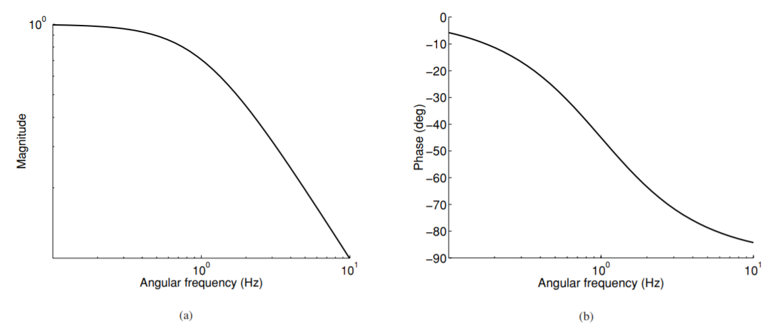
\includegraphics[width=0.8\linewidth]{../../Figures/Magnitude_Shift_Low_Pass.PNG}
    \caption{Bode plot of a first order linear system, such as the RC circuit of Fig. \ref{fig:RC_Circuits}.a) Magnitude and b) Phase as a function of input signal angular frequency $\omega$. Adapted from Textbook.}
    \label{fig:Filtering}
\end{figure}

We define the frequency $\omega_{cutoff} = \frac{1}{\tau}$ as the \textbf{cutoff frequency}.  The cutoff frequency is the frequency at which, either above or below (depending on if you are using a low pass or high pass filter), the power output of a circuit is reduced to \textbf{1/2 of the passband power} \footnote{Power, not amplitude. Remember that for an electrical circuit, power $P = \frac{V^2}{R}$}. This is equivalent to a voltage (or amplitude) reduction of 70.7\% of the passband, because voltage $V^2$ is proportional to power P. This happens to be close to -3 decibles and the cutoff frequency is frequency referred to as the -3dB point. In (Figure \ref{fig:Filtering}), it is set equal to 1.

Now let's look at a plot which really demonstrates how the response (output) of the input signal is reduced after filtering in figure \ref{fig:Filtering}. 

\begin{figure}[H]
    \centering
    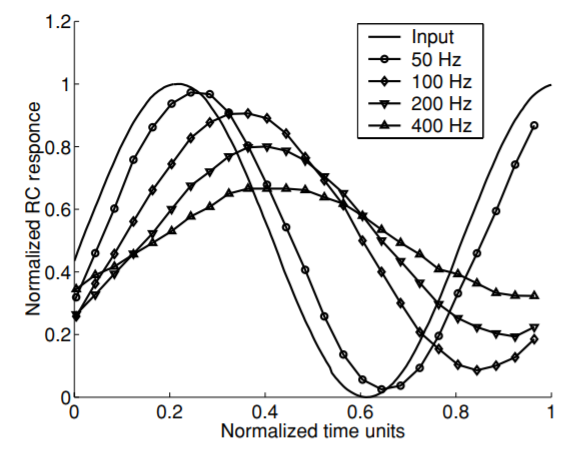
\includegraphics[width=0.55\linewidth]{../../Figures/Low_Pass_Filtering.PNG}
    \caption{Response of an RC low-pass filter ($R = 10M\ohm, C = 1nF$) to input sinusoids of different frequencies. The input signals have been normalized to unity, and the outputs have been normalized with respect to the input. The time axis has also been normalized so that the responses to all the frequencies could be presented on the same graph. Adapted from Textbook.}
    \label{fig:Filtering_2}
\end{figure}


The RC circuit of figure \ref{fig:RC_Circuits}.a allows sinusoidal
signals with frequencies lower than the cutoff frequency to pass virtually
unchanged. On the other hand, the frequency components of the input signals
that are above the cutoff frequency are attenuated. The phase lag between the
input and the output of the system increases with $\omega$ (see Figure \ref{fig:Filtering}.b) and saturates at 90 degrees. Figure \ref{fig:Filtering_2} shows experimental data measured from an RC lowpass filter with R = 10M$\ohm$ and C = 1nF . Sinuosoids of increasing
frequency were applied to the circuit and the corresponding responses were
measured. To show the effect of a range of input frequencies on the circuit’s
response, all the data are plotted on a normalized scale. The responses have
been normalized with respect to the input and time has been normalized to
unity. As expected, the output signal is attenuated as the input frequency
increases; and the phase lag between the input and output signals increases
with increasing frequency.

\paragraph{Summary about filters}
\begin{itemize}
    \item The figures we've just shown are for RC Low-Pass filters. The amplitude and power of the output signal decreases for high frequencies. 
    \item The time constant $\tau = RC$ determines what high and low frequencies are, it also determines the cutoff frequency (at which output power is halved)
    \item Cutoff frequency $\omega_{cutoff} = \frac{1}{RC}$
    \item CR circuit (figure \ref{fig:RC_Circuits}.b), is a high pass filter, which is just the same as we've shown but in reverse: it passes high frequencies and reduces low frequency. 
    \item You can build a \textit{band pass} filter from combining a high pass and low pass filter: the low pass will reduce all frequencies higher than your max desired frequency and the high pass will reduce all frequencies lower than your min desired frequency. 
    \item Why is this even useful? Imagine you're trying to process sound, like music for example, where you have some high frequency noise that is not your music (you barely hear it but it's there and alters your recording). Would be great if you could filter that out right? And only keep the frequencies of sound that are actually coming from the music (between ~10 and 3000 Hz). This is just one dumb example on the top of my mind of why filtering is useful, and we'll see in the next section applications in Neuromorphic Engineering. 
\end{itemize}



